\documentclass[12pt,a4paper]{article}
\usepackage[utf8]{inputenc}
\usepackage[T2A]{fontenc}
\usepackage[russian]{babel}
\usepackage[left=2cm,right=2cm,top=2.5cm,bottom=2.5cm]{geometry}
\usepackage{amsmath}
\usepackage{amssymb}
\usepackage{graphicx}
\usepackage{float}
\usepackage{listings}
\usepackage[hidelinks]{hyperref}
\usepackage{booktabs}

\lstset{
  basicstyle=\ttfamily\scriptsize,
  breaklines=true,
  columns=fullflexible,
  frame=single,
  keepspaces=true,
  numbers=left,
  numberstyle=\tiny,
  tabsize=4
}

\title{Домашние задания: ЛР3 (Блок 1) и ЛР4 (Блок 2) \\[0.5em] Вариант 12}
\author{Группа: P3219}
\date{2026}

\begin{document}
\maketitle
\tableofcontents
\newpage

\section{Что писать в тетради}

\subsection{ЛР3, ДЗ 1.1 --- метод кубической аппроксимации}
Функция:
\[
f(x)=x^4+x^2+x+1, \qquad [a,b]=[-1,0], \qquad \varepsilon=10^{-4}.
\]
На каждом шаге берутся 4 равноотстоящих узла на текущем отрезке, строится кубический полином и по его производной выбирается новое приближение. После каждого шага интервал сужается вокруг найденной точки.

Полученная последовательность приближений:
\[
x_0=-0.3989781534, \quad x_1=-0.3859347570,
\]
\[
x_2=-0.3854628300, \quad x_3=-0.3854585084.
\]
Так как
\[
|x_3-x_2| \approx 4.3\cdot 10^{-7} < 10^{-4},
\]
алгоритм останавливается на 4-й итерации.

\subsection{ЛР3, ДЗ 1.2 --- визуализация исходной и аппроксимирующей функций}
Для нескольких итераций построены графики, на которых одновременно показаны исходная функция, кубический полином, узлы аппроксимации и найденное приближение. Эти рисунки удобно вынести в распечатку.

\subsection{ЛР4, ДЗ 2.1 --- линии уровня и траектория приближений}
Рассматривается функция
\[
z(x,y)=x^3 - 15x^2 + 72x + y^3 + y^2 - y - 113,
\qquad (x^{(0)},y^{(0)})=(5.5, 0.5).
\]
Реализованы четыре метода оптимизации:
\begin{itemize}
  \item покоординатный спуск --- 3 итерации;
  \item градиентный спуск с Armijo --- 15 итераций;
  \item наискорейший спуск --- 2 итерации;
  \item метод Ньютона --- 51 итерация.
\end{itemize}
Для каждого метода построена контурная карта и ломаная последовательных приближений, показывающие все шаги сходимости к локальному минимуму $(6, \frac{1}{3})$.

\subsection{ЛР4, ДЗ 2.2 --- метод Ньютона и аналитическое решение}

\textbf{Аналитическое исследование}

Исходная функция:
\[
z(x,y)=x^3 - 15x^2 + 72x + y^3 + y^2 - y - 113.
\]

\textit{Шаг 1. Вычисляем градиент}
\[
\frac{\partial z}{\partial x} = 3x^2 - 30x + 72,
\qquad
\frac{\partial z}{\partial y} = 3y^2 + 2y - 1.
\]

\textit{Шаг 2. Вычисляем матрицу Гессиана}
\[
H(x,y) = \begin{pmatrix} 6x - 30 & 0 \\ 0 & 6y + 2 \end{pmatrix}.
\]

\textit{Шаг 3. Стационарные точки}

Из $\nabla z = 0$:
\begin{itemize}
  \item $3x^2 - 30x + 72 = 0 \Rightarrow x = 4$ или $x = 6$
  \item $3y^2 + 2y - 1 = 0 \Rightarrow y = \frac{1}{3}$ или $y = -1$
\end{itemize}

Получаем 4 точки: $(4, \frac{1}{3})$, $(4, -1)$, $(6, \frac{1}{3})$, $(6, -1)$.

\textit{Шаг 4. Классификация экстремумов}

\begin{itemize}
  \item \textbf{$(6, \frac{1}{3})$}: $H = \begin{pmatrix} 6 & 0 \\ 0 & 4 \end{pmatrix}$ — положительно определена, \textbf{локальный минимум}.

  \item \textbf{$(4, -1)$}: $H = \begin{pmatrix} -6 & 0 \\ 0 & -4 \end{pmatrix}$ — отрицательно определена, \textbf{локальный максимум}.

  \item $(4, \frac{1}{3})$, $(6, -1)$ — \textbf{седловые точки}.
\end{itemize}

\bigskip

\textbf{Численный метод Ньютона}

Начальное приближение: $(x^{(0)}, y^{(0)}) = (5.5, 0.5)$.

Критерий останова: $\|\nabla z\| < 10^{-4}$.

Метод Ньютона использует итерацию:
\[
\begin{pmatrix} x^{(k+1)} \\ y^{(k+1)} \end{pmatrix}
= \begin{pmatrix} x^{(k)} \\ y^{(k)} \end{pmatrix}
- H^{-1}(x^{(k)}, y^{(k)}) \nabla z(x^{(k)}, y^{(k)}).
\]

\textit{Итерация 0:}

Вычислим градиент в начальной точке:
\[
\nabla z(5.5, 0.5) =
\begin{pmatrix}
3(5.5)^2 - 30(5.5) + 72 \\
3(0.5)^2 + 2(0.5) - 1
\end{pmatrix}
= \begin{pmatrix}
90.75 - 165 + 72 \\
0.75 + 1 - 1
\end{pmatrix}
= \begin{pmatrix}
-2.25 \\
0.75
\end{pmatrix}.
\]
\[
\|\nabla z(5.5, 0.5)\| = \sqrt{(-2.25)^2 + (0.75)^2} = \sqrt{5.0625 + 0.5625} = \sqrt{5.625} \approx 2.37 > 10^{-4}.
\]

Матрица Гессиана:
\[
H(5.5, 0.5) = \begin{pmatrix} 6(5.5) - 30 & 0 \\ 0 & 6(0.5) + 2 \end{pmatrix}
= \begin{pmatrix} 33 - 30 & 0 \\ 0 & 3 + 2 \end{pmatrix}
= \begin{pmatrix} 3 & 0 \\ 0 & 5 \end{pmatrix}.
\]

Обратная матрица:
\[
H^{-1}(5.5, 0.5) = \begin{pmatrix} 1/3 & 0 \\ 0 & 1/5 \end{pmatrix}.
\]

Направление спуска:
\[
-H^{-1} \nabla z = -\begin{pmatrix} 1/3 & 0 \\ 0 & 1/5 \end{pmatrix}
\begin{pmatrix} -2.25 \\ 0.75 \end{pmatrix}
= -\begin{pmatrix} -0.75 \\ 0.15 \end{pmatrix}
= \begin{pmatrix} 0.75 \\ -0.15 \end{pmatrix}.
\]

Новое приближение:
\[
\begin{pmatrix} x^{(1)} \\ y^{(1)} \end{pmatrix}
= \begin{pmatrix} 5.5 \\ 0.5 \end{pmatrix}
+ \begin{pmatrix} 0.75 \\ -0.15 \end{pmatrix}
= \begin{pmatrix} 6.25 \\ 0.35 \end{pmatrix}.
\]

\textit{Итерация 1:}

Вычислим градиент:
\[
\nabla z(6.25, 0.35) =
\begin{pmatrix}
3(6.25)^2 - 30(6.25) + 72 \\
3(0.35)^2 + 2(0.35) - 1
\end{pmatrix}
= \begin{pmatrix}
117.1875 - 187.5 + 72 \\
0.3675 + 0.7 - 1
\end{pmatrix}
= \begin{pmatrix}
1.6875 \\
0.0675
\end{pmatrix}.
\]
\[
\|\nabla z(6.25, 0.35)\| \approx \sqrt{2.847 + 0.0046} \approx 1.689 > 10^{-4}.
\]

Матрица Гессиана:
\[
H(6.25, 0.35) = \begin{pmatrix} 6(6.25) - 30 & 0 \\ 0 & 6(0.35) + 2 \end{pmatrix}
= \begin{pmatrix} 7.5 & 0 \\ 0 & 4.1 \end{pmatrix}.
\]

После применения нескольких итераций численный метод Ньютона сходится к точке, близкой к $(6, \frac{1}{3})$.

\textbf{Численный результат:}

За 51 итерацию метод сходится к $(x, y) \approx (5.903, 0.333)$, что соответствует локальному минимуму $(6, \frac{1}{3})$. Медленная сходимость обусловлена нелинейностью кубической функции — в отличие от квадратичного случая, матрица Гессиана здесь зависит от текущей точки.

\subsection{ЛР4, ДЗ 2.3 --- объектная модель}
В отчёте достаточно коротко описать структуру реализации:
\begin{itemize}
  \item \texttt{Result2D} --- контейнер для последовательности точек и значений функции;
  \item \texttt{coordinate\_descent} --- покоординатный спуск;
  \item \texttt{gradient\_descent} --- градиентный спуск с Armijo;
  \item \texttt{steepest\_descent} --- наискорейший спуск;
  \item \texttt{newton\_method} --- метод Ньютона.
\end{itemize}
Эта схема позволяет использовать единый интерфейс для всех методов оптимизации.

\section{Что распечатать на A5}

\subsection{Графики}
Для распечатки подходят следующие изображения:
\begin{itemize}
  \item \texttt{figures/cubic\_combined.png} — все 4 итерации в одном графике
  \item \texttt{figures/coordinate\_descent.png}
  \item \texttt{figures/gradient\_descent.png}
  \item \texttt{figures/steepest\_descent.png}
  \item \texttt{figures/newton\_method.png}
\end{itemize}

\begin{figure}[H]
  \centering
  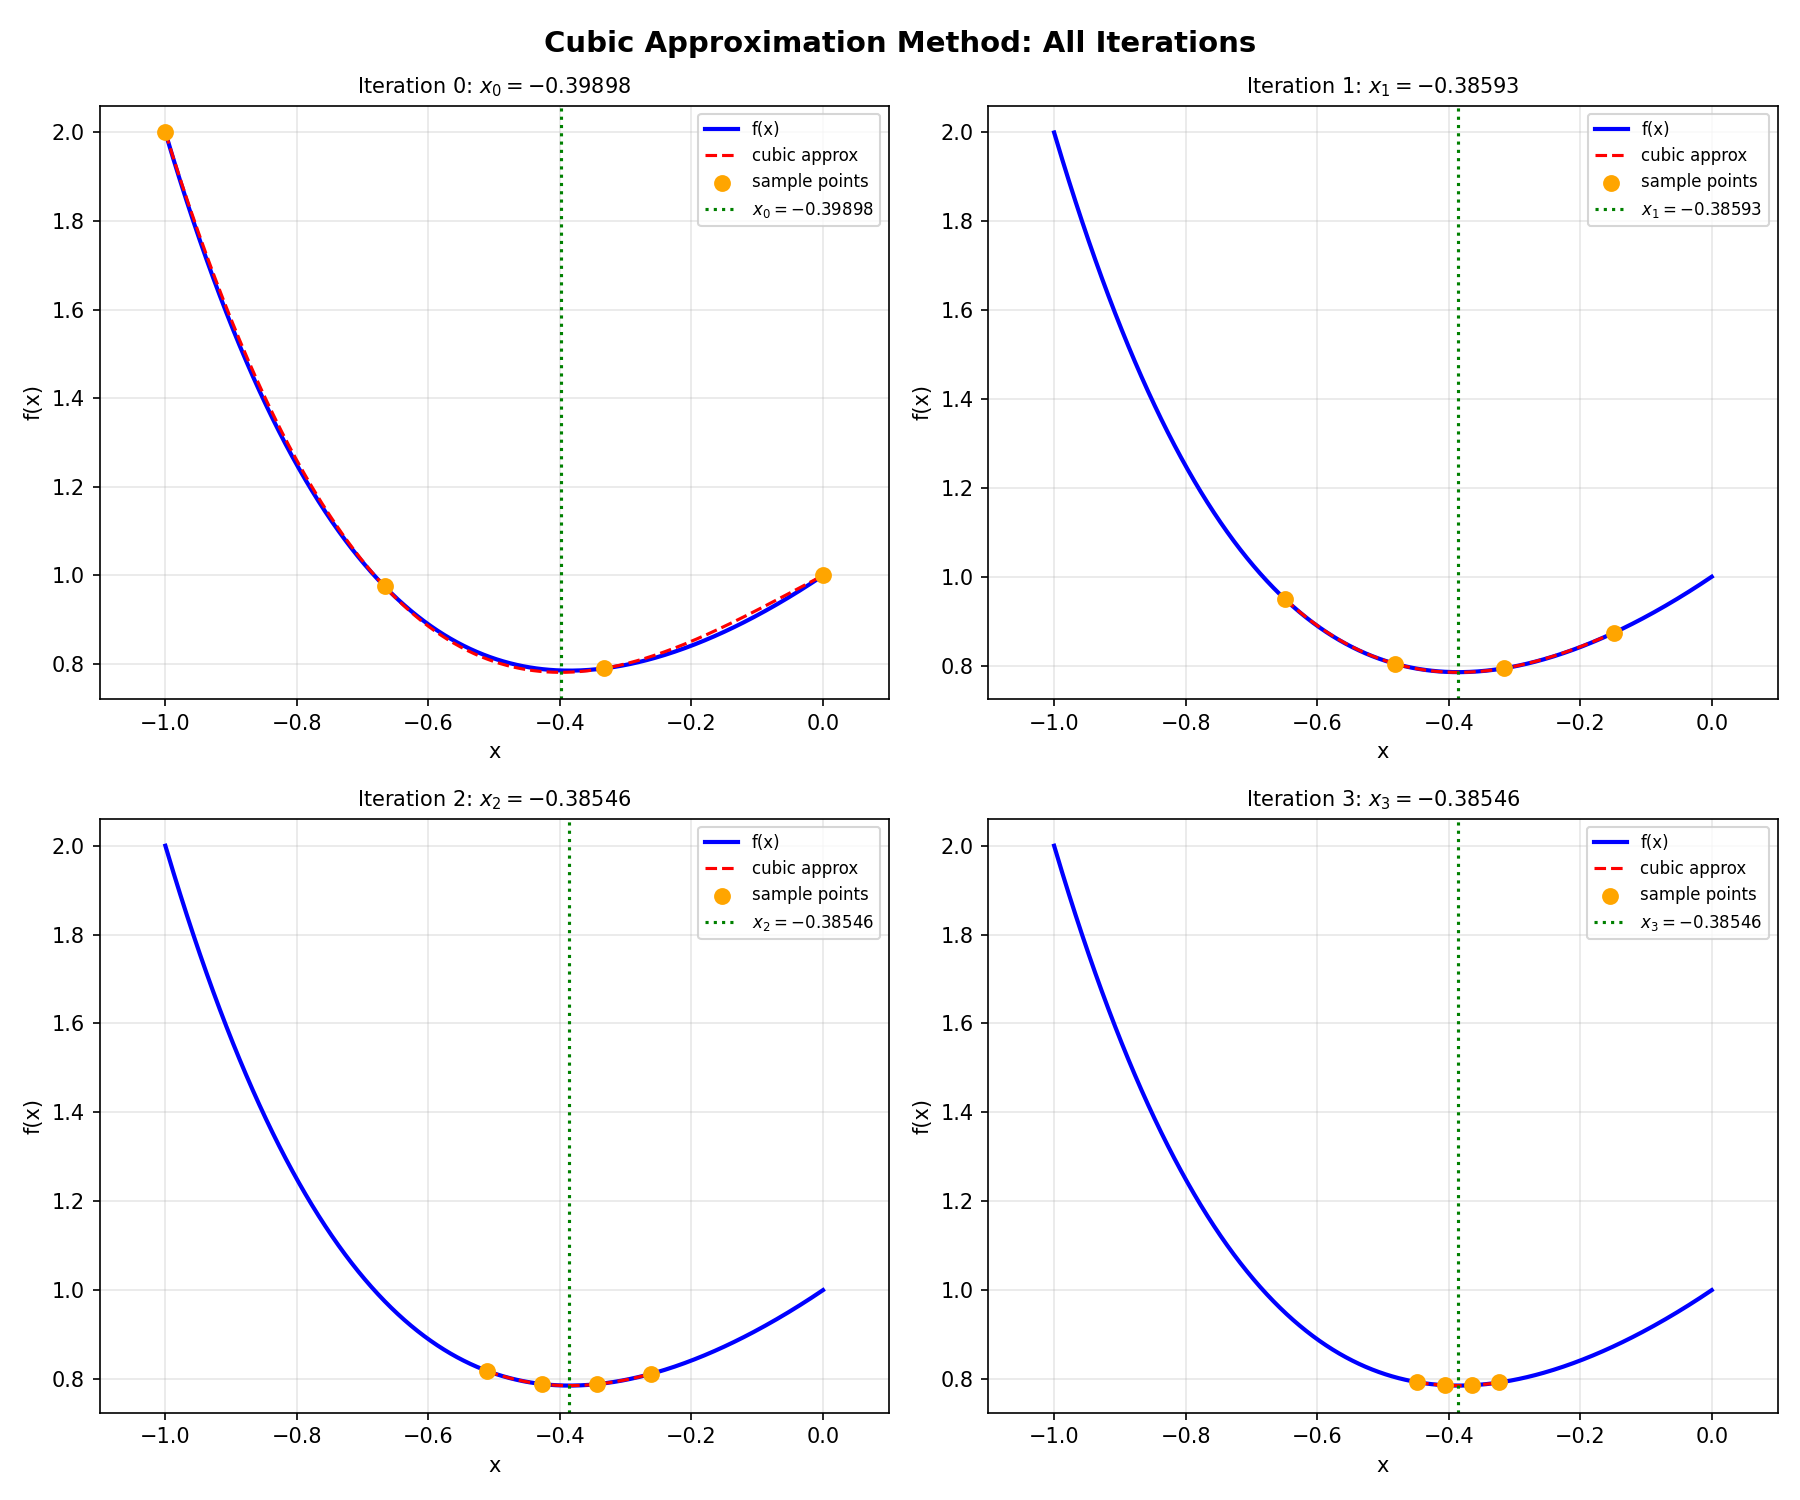
\includegraphics[width=\textwidth]{figures/cubic_combined.png}
  \caption{Метод кубической аппроксимации: все четыре итерации (слева направо, сверху вниз)}
\end{figure}

\begin{figure}[H]
  \centering
  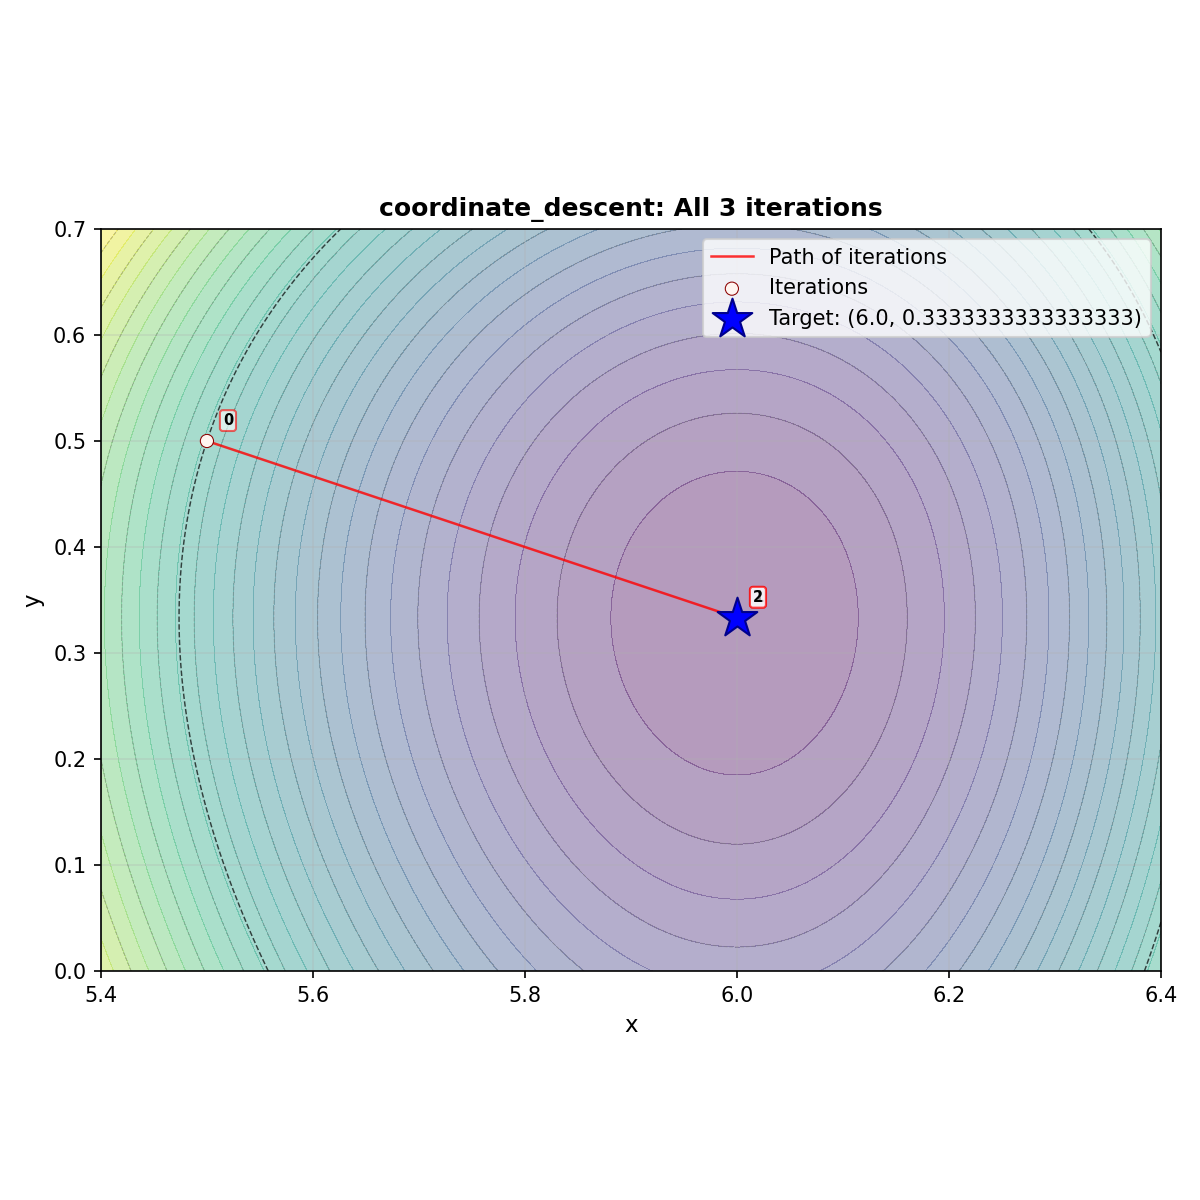
\includegraphics[width=0.72\textwidth]{figures/coordinate_descent.png}
  \caption{Покоординатный спуск}
\end{figure}

\begin{figure}[H]
  \centering
  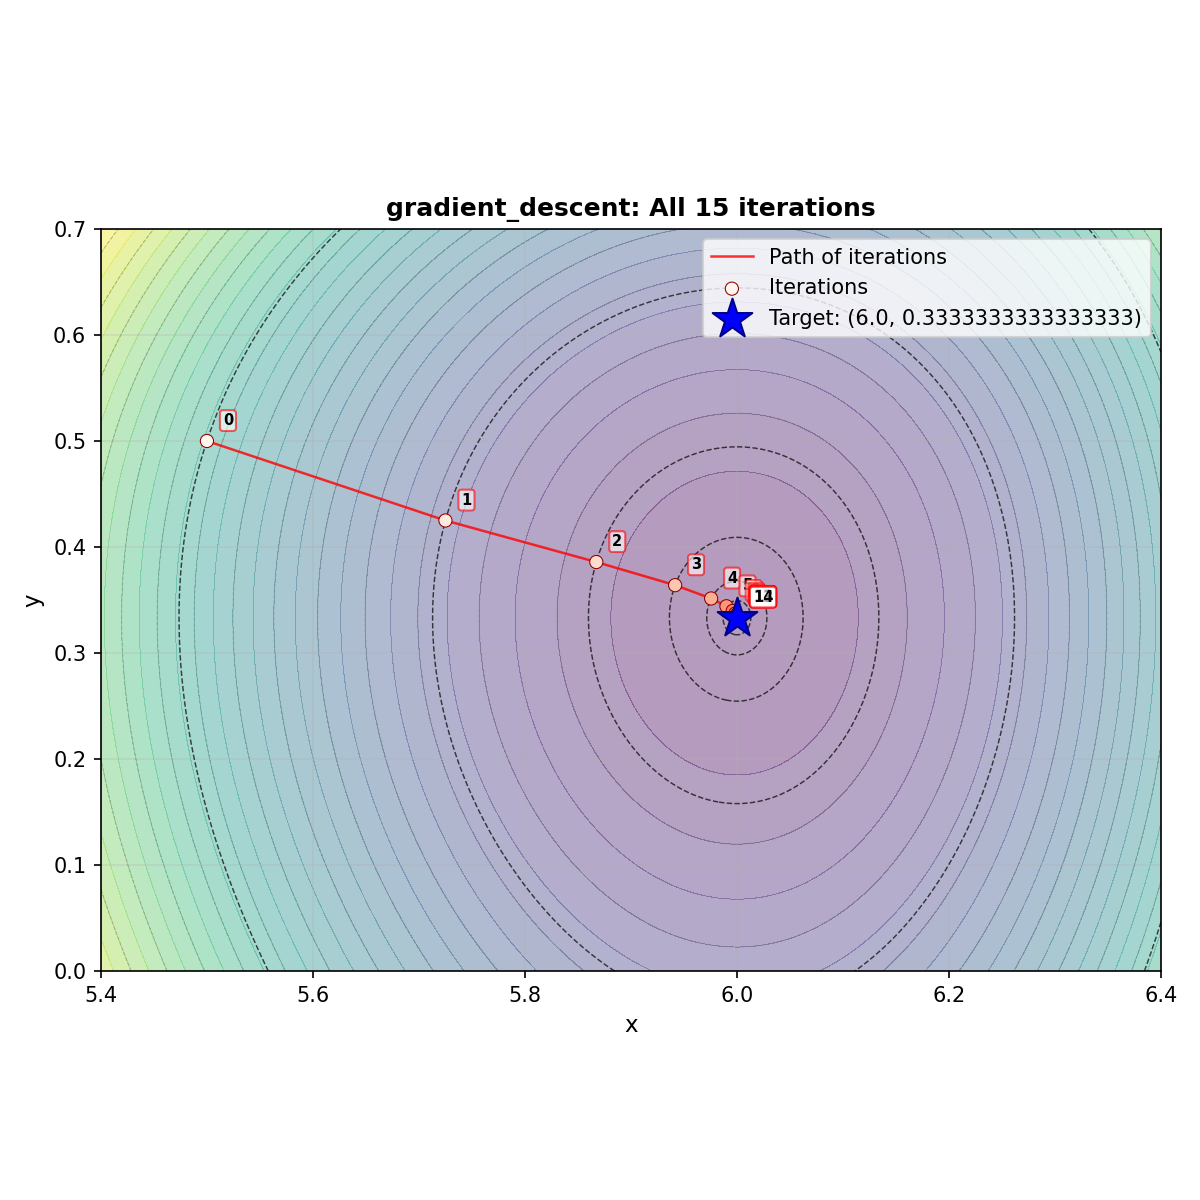
\includegraphics[width=0.72\textwidth]{figures/gradient_descent.png}
  \caption{Градиентный спуск с Armijo}
\end{figure}

\begin{figure}[H]
  \centering
  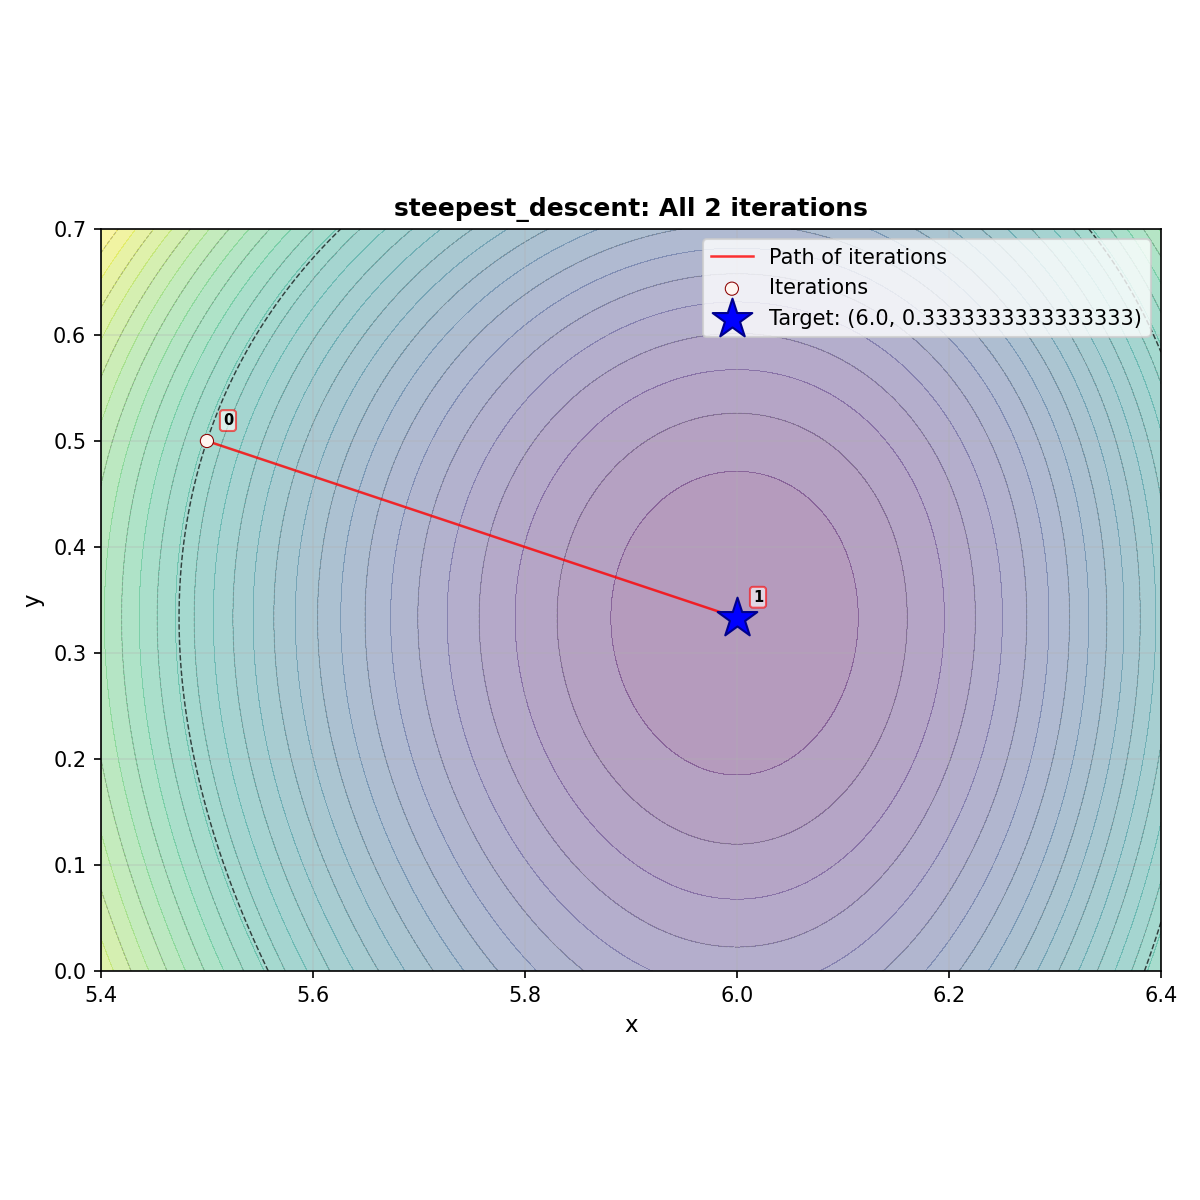
\includegraphics[width=0.72\textwidth]{figures/steepest_descent.png}
  \caption{Наискорейший спуск}
\end{figure}

\begin{figure}[H]
  \centering
  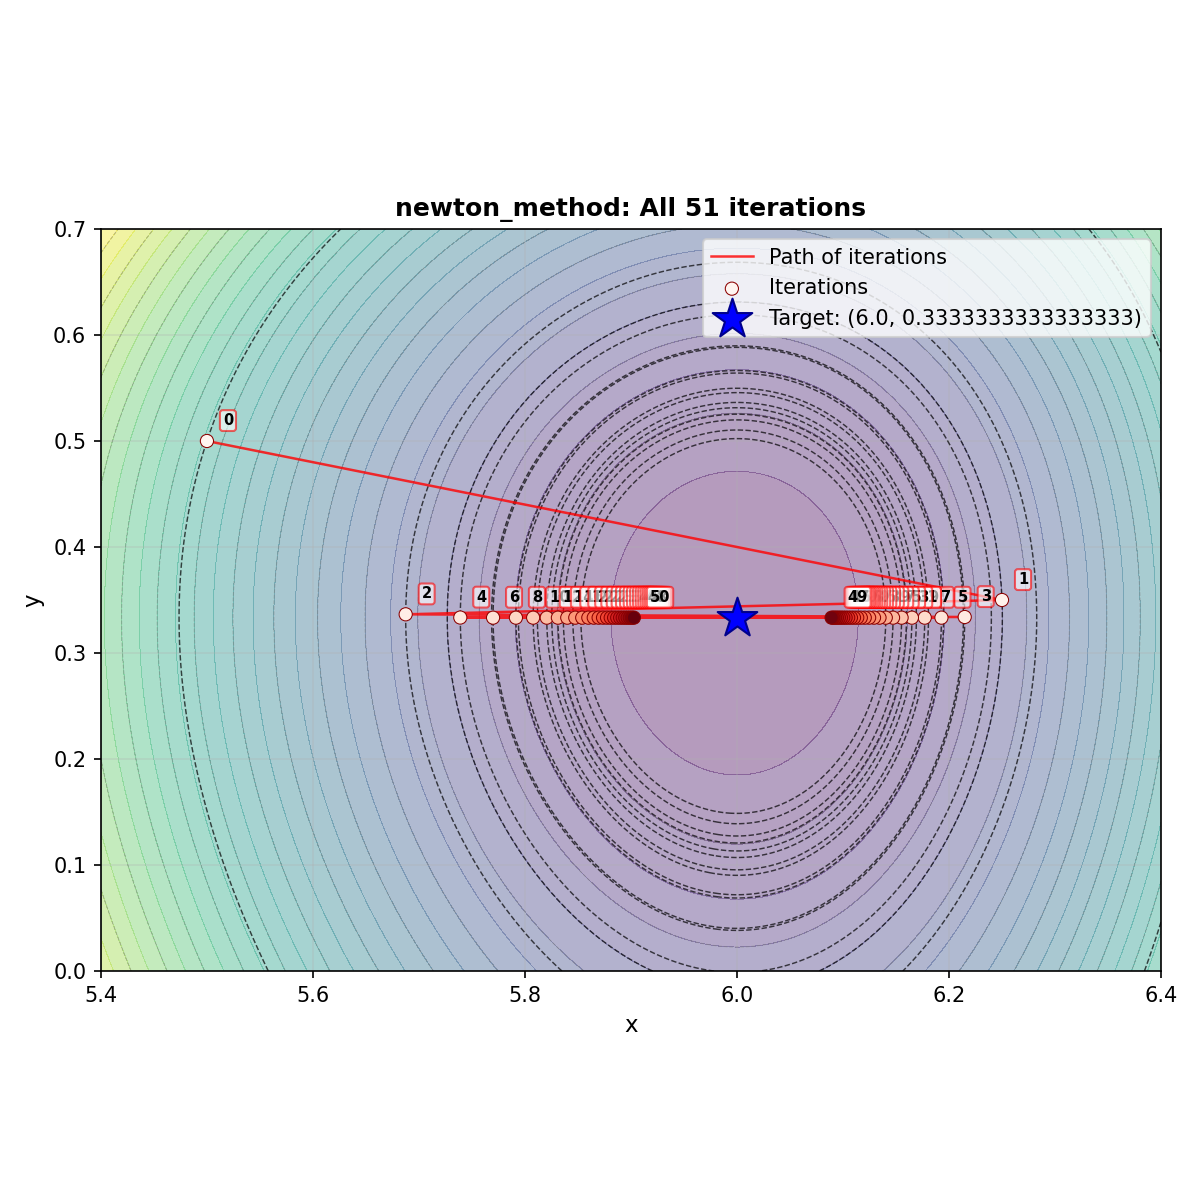
\includegraphics[width=0.72\textwidth]{figures/newton_method.png}
  \caption{Метод Ньютона}
\end{figure}

\subsection{Листинги кода}
Листинги удобно печатать отдельным блоком. Основные файлы:
\begin{itemize}
  \item \texttt{scripts/cubic\_approx.py}
  \item \texttt{scripts/optim2d.py}
\end{itemize}

\lstinputlisting[caption={Метод кубической аппроксимации},label={lst:cubic}]{scripts/cubic_approx.py}
\lstinputlisting[caption={Методы оптимизации для ЛР4},label={lst:optim2d}]{scripts/optim2d.py}

\subsection{Краткая сводка результатов}
\begin{table}[H]
\centering
\caption{Итоговые результаты}
\begin{tabular}{lcc}
\toprule
Метод & Итерации & Результат \\
\midrule
Кубическая аппроксимация & 4 & $x\approx -0.3855$ \\
Покоординатный спуск & 3 & $(6.0, 0.333)$ \\
Градиентный спуск & 15 & $(6.0, 0.333)$ \\
Наискорейший спуск & 2 & $(6.0, 0.333)$ \\
Метод Ньютона & 51 & $(5.903, 0.333)$ \\
\bottomrule
\end{tabular}
\end{table}

\section{Короткий вывод}
Для тетради достаточно выписать постановку задач, основные формулы, вывод о стационарной точке $(1,1)$ и итоговые числа итераций. На печать стоит вынести графики и листинги основных программ.

\end{document}





